\chapter{Dynamic parallel \hp-adaptive \glsfmtlongpl{fem}}
\label{ch:dynamic}
\glsresetall

Up to this point, we have only dealt with static \hp-adaptive meshes, in which the grid resolution and the distribution of finite elements is prescribed from the beginning. % Those can be used for multi-physics applications, in which different characteristics can be assigned to certain parts of the domain using dedicated finite elements.
However, the key feature of \hp-adaptive methods is the dynamic distribution of these attributes. The goal is to reduce the overall error of the approximation on the basis of the complexity of the current state of the solution. With dynamic methods, meshes can be tailored to a specific problem iteratively with so called SOLVE-ESTIMATE-MARK-REFINE cycles: After solving the problem on a coarse mesh, it will be adapted based on an error estimate several times, as we will demonstrate in Ch.~\ref{ch:results}. Also, time dependent problems benefit from dynamic adaptation, in which mesh attributes will be adjusted on the basis of the solution that evolves in time, for example, for heat transfer \textcite{dealiistep-26} and fluid flow problems \textcite{dealiistep-31}.

In practice, we distinguish between two ways of imposing these \hp-adaptive methods: either manually or automatically. The combination of both \h- and \p-adaptation poses new challenges. We will present these issues in this chapter along with algorithms to automatically determine which regions to adapt and which type of adaptation to impose.

First, considerations regarding the implementation of \hp-adaptivity will be presented. We then propose methods to automatically decide which cells to adapt and how by providing corresponding adaptation and decision strategies. The presented strategies are intended for general purposes and are based on error estimation, error prediction and smoothness estimation. It is conceivable to tailor strategies around particular observables of individual problems, which is not subject of this dissertation. Furthermore, dynamic changes on the mesh require data exchange between processes, which we describe in the end.

New features for \hp-adaptation as well as a generalized interface have been introduced in the \dealii{} library \textcite{dealii920} during working on this dissertation. A development log on all features introduced in the context of dynamic \hp-adaptive \glspl{fem} can be found here \cite{dealiiissue7515}.



\section{Realization of \hp-adaptation}
\label{sec:adaptation}

For \hp{}-adaptive methods we need to find ways to prescribe which cells are subject to which kind of adaptation. This grants awareness on how the mesh will change if adaptation is executed.

To indicate that adaptation is about to happen, we introduce general flags for refinement and coarsening, respectively. We are left to distinguish between \h- and \p-adaptation. To do this, we specify so called \textit{future finite element} indices that determine the finite element that will be associated to that particular cell after adaptation has been performed. If such a future finite element is defined on marked cells, \p-adaptation will be performed, while cells will be \h-adapted if none is specified. This approach offers full flexibility to let either users decide manually how to adapt, but also provides a sufficient interface for an automatic specification of these mesh attributes.

To determine the extent to which cells change during the adaptation process, the affected cell properties have to be hierarchically ordered. While for \h-adaptive methods, a grid hierarchy naturally evolves from the underlying tree or forest data structure, this is not necessarily the case for \p-adaptation. Here, a hierarchy needs to be provided for the collection of finite elements, so that we can assign superior and subordinate elements in case of \p-refinement or \p-coarsening, respectively. For example, we arrange Lagrangian finite elements by their polynomial degree in ascending order with the largest degree on the highest level.

Executing \h-adaptation on a \p-adapted mesh reveals another challenge. We need to find a suitable finite element on cells that will be \h-adapted. During \h-refinement, we can easily choose the finite element from the parent cell for all of its children, but for \p-coarsening, the choice is not trivial. From all cells that are going to be \h-coarsened, we pick the one finite element for the parent cell from those assigned to its children that encapsulates all of them. With simultaneous \h- and \p-adaptation, future finite elements will be considered instead of the active one. This conforms to the finite element domination logic that has been introduced by \textcite{bangerth2009} and is described in Sec.~\ref{sec:prerequisities}. An example on how finite elements are distributed during \hp-adaptation is shown in Fig.~\ref{fig:adaptation}.

\begin{figure}
\begin{subfigure}{.5\textwidth}
  \centering
  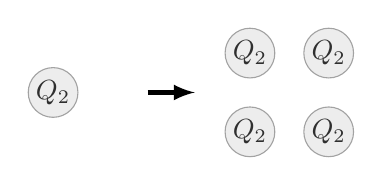
\begin{tikzpicture}[>=latex]
\def\Length{1}
\def\Radius{0.07}

% pre refinement
\LagrangeCell{0}{0}{2*\Length}{\Radius}{2}
  {{,,,,,,,,}};
\node[circle, draw=gray, fill=gray!20, inner sep=1pt, opacity=0.7, text opacity=0.8] at (\Length,\Length) {$Q_2$};

% arrow
\draw[->,ultra thick] (2.2*\Length,\Length) -- (2.8*\Length,\Length);

% post refinement
\LagrangeCell{3*\Length}{0}{\Length}{\Radius}{2}
  {{,,,,,,,,}};
\node[circle, draw=gray, fill=gray!20, inner sep=1pt, opacity=0.7, text opacity=0.8] at (3.5*\Length,0.5*\Length) {$Q_2$};

\LagrangeCell{4*\Length}{0}{\Length}{\Radius}{2}
  {{,,,,,,,,}};
\node[circle, draw=gray, fill=gray!20, inner sep=1pt, opacity=0.7, text opacity=0.8] at (4.5*\Length,0.5*\Length) {$Q_2$};

\LagrangeCell{3*\Length}{\Length}{\Length}{\Radius}{2}
  {{,,,,,,,,}};
\node[circle, draw=gray, fill=gray!20, inner sep=1pt, opacity=0.7, text opacity=0.8] at (3.5*\Length,1.5*\Length) {$Q_2$};

\LagrangeCell{4*\Length}{\Length}{\Length}{\Radius}{2}
  {{,,,,,,,,}};
\node[circle, draw=gray, fill=gray!20, inner sep=1pt, opacity=0.7, text opacity=0.8] at (4.5*\Length,1.5*\Length) {$Q_2$};
\end{tikzpicture}
  \caption{\hp-refinement.}
\end{subfigure}
\begin{subfigure}{.5\textwidth}
  \centering
  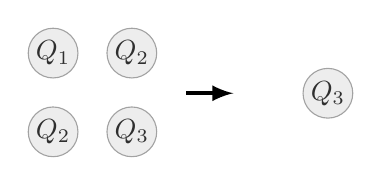
\begin{tikzpicture}[>=latex]
\def\Length{1}
\def\Radius{0.07}

% pre coarsening
\LagrangeCell{0}{0}{\Length}{\Radius}{2}
  {{,,,,,,,,}};
\node[circle, draw=gray, fill=gray!20, inner sep=1pt, opacity=0.7, text opacity=0.8] at (0.5\Length,0.5\Length) {$Q_2$};

\LagrangeCell{\Length}{0}{\Length}{\Radius}{3}
  {{,,,,,,,,,,,,,,,}};
\node[circle, draw=gray, fill=gray!20, inner sep=1pt, opacity=0.7, text opacity=0.8] at (1.5\Length,0.5\Length) {$Q_3$};

\LagrangeCell{0}{\Length}{\Length}{\Radius}{1}
  {{,,,}};
\node[circle, draw=gray, fill=gray!20, inner sep=1pt, opacity=0.7, text opacity=0.8] at (0.5\Length,1.5\Length) {$Q_1$};

\LagrangeCell{\Length}{\Length}{\Length}{\Radius}{2}
  {{,,,,,,,,}};
\node[circle, draw=gray, fill=gray!20, inner sep=1pt, opacity=0.7, text opacity=0.8] at (1.5\Length,1.5\Length) {$Q_2$};

% arrow
\draw[->,ultra thick] (2.2*\Length,\Length) -- (2.8*\Length,\Length);

% post coarsening
\LagrangeCell{3*\Length}{0}{2*\Length}{\Radius}{3}
  {{,,,,,,,,,,,,,,,}};
\node[circle, draw=gray, fill=gray!20, inner sep=1pt, opacity=0.7, text opacity=0.8] at (4*\Length,\Length) {$Q_3$};
\end{tikzpicture}
  \caption{\hp-coarsening.}
\end{subfigure}
\caption[Inheritance of cell characteristics through \hp-adaptation.]{Inheritance of cell characteristics through \hp-adaptation. With \hp-refinement, all children will be associated with the parent finite element, while during \hp-coarsening, the finite element space chosen on the parent cell encapsulates all those of its children ($Q_1 \subset Q_2 \subset Q_3$).}
\label{fig:adaptation}
\end{figure}
\section{Decision criteria}
\label{sec:decision}

A common observation is that increasing the grid resolution or the polynomial degree of the basis functions will decrease the difference between the finite element approximation $u_\text{hp}$ and the actual solution $u$.

In fact, the impact of these adaptation techniques on the error is well understood. \textcite[Thm.~3.4]{babuska1990} determined an upper bound for the error that depends both on the cell diameter $h$ and the polynomial degree $p$:
\begin{align}
\label{eq:errorbound_hp} \left\|e_\text{hp}\right\|_{H^{1}(\Omega)} &\leq C \, h^{\mu} \, p^{-(m-1)} \, \|u\|_{H^{m}(\Omega)} \,\text{,}
\end{align}
where $e_{hp} = u - u_\text{hp}$ denotes the error function, $m$ is a measure for the regularity of the solution $u$, $C$ is a constant dependent on $m$, and $\mu = \min \left(p, m - 1\right)$.

These modifications do not have to happen uniformly on a global scale, but can be applied locally, since the global error consists of the local ones of each cell $K$:
\begin{align}
\label{eq:error_sum} \left\|e_\text{hp}\right\|_{H^1(\Omega)}^2 = \sum\limits_{K \in \Omega} \left\|e_\text{hp}\right\|_{H^1(K)}^2 \,\text{.}
\end{align}
Thus it all comes down to find those sections that have a significant contribution to the global error, and mitigate their impact by local adaptation. \textcite[Thm.~5.1]{guo1986} predict exponential convergence with the number of \glspl{dof} $n_\text{dofs}$ on a suitable \hp-adapted mesh:
\begin{align}
\label{eq:errorbound_exp} \left\|e_\text{hp}\right\|_{H^{1}(\Omega)} &\leq C \, \exp\left(- b \, n_\text{dofs}^{1 / 3}\right) \,\text{,}
\end{align}
where constants $b > 0$ and $C$ are both independent of $n_\text{dofs}$.

With sufficient information about the investigated scenario, an \hp-adaptive grid can be tailored to its specifics manually. However, grid adjustments by hand may not be optimal. Furthermore, not all peculiarities about the scenario are generally known in advance, which is especially the case for problems with complex geometries and time dependent ones.

Hence we need to elaborate on algorithms to automatically decide which subsets of the domain qualify for adaptation. With this technique, we typically set up a coarse mesh along with basis functions of a low polynomial degree and obtain a tailored mesh after several adaptation iterations.

In this section, we present different ways to identify areas whose adaptation will be most profitable, and to choose the most beneficial type of adaptation. A selection of strategies for the latter have been reviewed and compared in detail by \textcite{mitchell2014}. We present a subset of their recommendations in terms of performance and applicability.



\subsection{Adaptation strategies}
\label{ssec:strategy}

With these indicators, we


We will decide on the basis of criteria for every cell which ones will be considered to be adapted. Typically errors or their estimates. Other indicators involve predicted errors or smoothness indicators which will be presented in the following sections.

\textcite[Sec.~5.2]{bangerth2003} describe different strategies, from which we present a commonly used selection.



So called fixed-error-reduction or fixed-fraction strategy takes that subset of cells whose indicators

with the that accumulated for a certain fraction of the error

This strategy only makes sense when the global sum of indicators actual has , for example local errors contribute to the global error in a global sum.

leads to optimal meshes


In practise, we need to find the maximum and minimum over all indicators, and interpolate the corresponding thresholds. In parallel, we have to do find a global maximum and minimum over all participating processors. And find a cer



So called fixed-rate or fixed-number strategy takes a predefined fraction of cells with the highest and lowest indicators, which will be considered for either refinement or coarsening, respectively. This allows us to predict the growth of cells, but may not lead to an optimal mesh since more cells than necessary may be adapted.

In practise, we need a binary search 

For parallel computations, we need a binary search. We will use the one presented by \textcites[Sec.~3.1]{burstedde2008}[Sec.~5.1]{bangerth2012}.



to find the maximum and minimum over all indicators, and interpolate the corresponding thresholds.





First, we need to identify those regions of the domain with the highest or least contribution to the global error, and we want to adapt these regions locally.

With these indicators, we are able to identify those regions of the domain with the highest or least contribution to the global error. We want to adapt these regions locally.



\subsection{Error estimation}
\label{ssec:estimation}

The determination of the error for our finite element approximation requires the actual solution to be at our disposal. However, this is not the case in general, and we need to come up with an alternative measure.

\textcite{kelly1983} worked out an error estimator for the generalized Poisson equation $-\nabla \cdot \left( a \nabla u \right) = f$, where $a$ is a function usually describing material characteristics. They determined an upper bound $\eta_K$ for the error on each cell by balancing the gradient of the finite element approximation $u_\text{hp}$ on all faces $F$ of the cell's boundary:
\begin{align}
\label{eq:kelly} \|e_\text{hp}\|_{H_1(\Omega)}^2 &\leq C \sum\limits_{K \in \Omega} \eta_K^2 &&\text{with}&  \eta_K^2 &= \sum\limits_{F \in \partial K} c_F \int\limits_{F} \left[ a \, \frac{\partial u_\text{hp}}{\partial n} \right]^2 \differential{o} \,\text{,}
\end{align}
where $C$ is independent of the solution, but depends on $a$, and
\begin{align*}
\left[ a \, \frac{\partial u_\text{hp}}{\partial n} \right] = \left. a \, \frac{\partial u_\text{hp}}{\partial n_K} \right|_K + \left. a \, \frac{\partial u_\text{hp}}{\partial n_J}\right|_J
\end{align*}
denotes the jump of the approximation's gradient on the face between two adjacent cells $K$ and $J$. Hence \textcite{ainsworth1997a} attribute this estimator to the class of gradient recovery estimators.

The constant $c_F$ depends on the characteristics of each individual face of the cell. \textcite{kelly1983} originally used the constant $c_F = \frac{h_K}{24 \, a_\text{min} \, p_K}$ on each face, on which we determine the minimum $a_\text{min}$ of the given function. Here, $h_K$ and $p_K$ denote both cell diameter and polynomial degree of the finite element on cell $K$, respectively. \textcite{davydov2017} proposed a different constant for \hp-adaptive \gls{fem}: They recommend $c_F = \frac{h_F}{2 \, a_\text{min} \, p_F}$ with $h_F$ the face diagonal and $p_F = \max\left(p_K, p_J\right)$ the largest polynomial degree of adjacent elements $K$ and $J$ on this particular face.

This estimator has been worked out for the Poisson equation, but has proven its applicability on other problems as well, where this is no longer meant to be an estimator, but rather an error indicator\todo{cite deal.II kelly error estimator website}.

The error estimator is already implemented in \dealii{}. \todo{cite deal.II kelly error estimator website}

We will use these error estimates to decide w. We are still left to decide which type of adaptation we want to apply, i.e.\@ \h-adaptation or \p-adaptation.



\subsection{Error prediction}
\label{ssec:prediction}

\cite{babuska1990} determined upper error bounds for numerical solutions based the distribution of finite elements. Both mesh resolution and polynomial degrees of the basis functions have a different, yet quantifiable influence on the error leading to Eq.~(\ref{eq:errorbound_hp}).

Their findings are valid not only for the numerical solution on a global scope, but on subsets of the domain as well. Local changes by \h- and \p-adaptation will thus result in different local error bounds. This motivates a strategy to locally decide which type of adaptation to impose based on the refinement history which has been proposed by \textcite{melenk2001}: We can predict how the current error will change whenever certain areas of our domain are considered for adaptation in the following iteration. These predicted error estimates allow us to decide whether the choice of adaptation in the previous step was justified, and provide the foundation for it on the next one.

We determine how the error bounds on two different distributions of finite elements will change by calculating their ratio. For this, we assume that both the actual error and its upper bound change with the same rate, which allows us to equate both ratios. We further assume that the solution is sufficiently regular ($m \gg p$). The ratio of errors then reads:
\begin{align}
\label{eq:errorratio_hp} \frac{||e_{h_f p_f}||_{H^{1}(K)}}{||e_{h_a p_a}||_{H^{1}(K)}} = \frac{h_f^{p_f}}{h_a^{p_a}} \, \left(\frac{p_f}{p_a}\right)^{-(m-1)} \,\text{,}
\end{align}
where subscripts $a$ and $f$ denote the finite element that is currently active or will be active after adaptation, respectively.

If we only consider \h-adaptation and leave the polynomial degree of the basis function unchanged ($p_f = p_a \equiv p$), we end up with the classical error bound \todo{cite}:
\begin{align}
\label{eq:errorratio_h} \frac{||e_{h_f p}||_{H^{1}(K)}}{||e_{h_a p}||_{H^{1}(K)}} = \left( \frac{h_f}{h_a} \right)^p \,\text{.}
\end{align}

However, if only \p-adaptation is considered and we keep the domain unchanged ($h_f = h_a \equiv h$), the ratio of errors still depends on the regularity of the actual solution which is not at our disposal in general.
\begin{align}
\label{eq:errorratio_p} \frac{||e_{h p_f}||_{H^{1}(K)}}{||e_{h p_a}||_{H^{1}(K)}} = h^{p_f - p_a} \, \left(\frac{p_f}{p_a}\right)^{-(m-1)}
\end{align}
Following the considerations of \cite{melenk2001}, we expect \p-adaptation to change the error exponentially with the increment of the polynomial degree
\begin{align}
\label{eq:errorratio_p_exp} \frac{||e_{h p_f}||_{H^{1}(K)}}{||e_{h p_a}||_{H^{1}(K)}} \simeq c^{p_f - p_a} \,\text{,}
\end{align}
where $c$ is a constant independent of the cell diameter $h$.

We suggest a similar approach for the hp-adaptation case as well. The above ratio assumes that the underlying mesh has not been changed. We thus identify Eq.~(\ref{eq:errorratio_p_exp}) with an unaltered cell diameter ($h \equiv h_a$) in Eq.~(\ref{eq:errorratio_hp}) resulting in:
\begin{align}
\label{eq:errorratio_hp_exp} \frac{||e_{h_f p_f}||_{H^{1}(K)}}{||e_{h_a p_a}||_{H^{1}(K)}} \simeq \left( \frac{h_f}{h_a} \right)^{p_f} \, c^{p_f - p_a} \,\text{.}
\end{align}
We will take this factor in all following considerations to predict how errors will change.

% ----------

% underscore
Again division on multiple cells in case of h-refinement.

For h-coarsening or hp-coarsening, we need to take special care. And h-coarsening involves summing up. Note that we take the new polynomial degree here.
\begin{align}
Some other nice formula hp coarsening
\end{align}
For pure h coarsening we consider
\begin{align}
Some other nice formula h coarsening
\end{align}

% start from here

All above relations not only hold for the whole domain $\Omega$, but also qualify for local adaptation on subsets of it, i.e.\@ any cell $K \in \Omega$. We write introduce control parameters

we need to subdivide it into it's children, thus

Isotropic refinement with quadrilaterals in two and hexahedrals in three dimensions.

We take
Nothing changes
\begin{align}
\label{eq:nothing} ||e_{h p}||_{H^1(K)} \simeq \gamma_n \, ||e_{h p}||_{H^1(K)}
\end{align}
with a control parameter \(\gamma_n = 1\).

p adaptation
\begin{align}
\label{eq:p_adaptation} ||e_{h p_f}||_{H^1(K)} \simeq \gamma_p^{p_f-p_a} \, ||e_{h p_a}||_{H^1(K)}
\end{align}
with a control parameter \(\gamma_p = \sqrt{0.1}\) chosen to be in accordance with \cite{melenk2001} and \cite{mitchell2014}.

hp refinement
\begin{align}
\label{eq:hp_refinement} ||e_{h_f p_f}||_{H^1(K_c)} \simeq \gamma_h \, n_c^{-1} \, 0.5^{p_f} \, \gamma_p^{p_f - p_{a_c}} ||e_{h_a p_a}||_{H^1(K)}
\end{align}
with control parameter \(\gamma_h = 1\).

hp coarsening
\begin{align}
\label{eq:hp_coarsening} ||e_{h_f p_f}||_{H^1(K)} \simeq \sum\limits_{c} \gamma_h^{-1} \, 2^{p_f} \, \gamma_p^{p_f - p_{\text{a}_c}} ||e_{h_{a_c} p_{a_c}}||_{H^1(K_c)}
\end{align}

% ---------

We now have an algorithm to predict the error for the next adaptation step on basis of the current one. We are left to find a suitable criterion on how to use it to actually decide .

The original idea of \cite{melenk2001} was to compare  for \h-refinement.
The idea behind this is that

We enhanced this approach for \h-coarsening
Similarly for coarsening, we can do this.

Another approach would be to treat the difference of predicted and estimated error as an indicator for each cell. From all cells that would be refined, we will consider those with the greatest values for p-refinement and the others for h-refinement. Analougously, those cells with the least difference will be \p-coarsened, while the

The error predictor has been implemented in the \dealii library as part of this dissertation. A development log can be found here.



\subsection{Smoothness estimation}
\label{ssec:smoothness}

Text.

\cite{mavriplis1994} introduced with the Legendre coefficient decay..


\cite{bangerth2009} introduced Fourier coefficient decay.
\section{Global data transfer}
\label{sec:transfer}

%For parallel \gls{fem}, we need to communicate data between processes in different stages of the application. The generation and modification of the distributed grid requires communication on all participating procceses. We already pointed out communication during the \gls{dof} enumeration process. The solution of the linear equation system also needs communication.

%Within the \dealii{} library, we rely on the parallel implementation of third party libraries at a lot of stages. All communication during the solution process will be made with parallel linear algebra libraries, i.e.\@ \petsc{} \textcite{petsc3124} and \trilinos{} \textcite{trilinos12181}. All operations on grid distribution is out-sourced to our oracle, which is \pforest{} \textcite{p4est22}.

%For parallel \gls{fem}, we need to communicate data between processes in different stages of the application. %One of the stages involves...

A major requirement for a general parallel \hp-adaptive \gls{fem} application is the ability to transfer data from the entirety of all cells or even the complete finite element approximation across adapted meshes. This is especially the case for time dependent or nonlinear problems, in which the solution of a problem on a recently adapted mesh depends on the finite element approximation of the preceding iteration from the previous mesh.

% --- Data preparation ---

%Whenever \h-adaptation is additionally involved,

%we need to collect all data before and unroll it after grid adaptation has been transformed on all locally owned cells. This process is similar to the sequential case and

%Compared to all point-to-point communication

% --- Fixed / Variable size transfer ---

In sequential and parallel applications with shared memory, each process has access to the complete memory set. However in \gls{hpc} applications with distributed memory, we need to transfer data on cells from processes that have previously owned them to processes that will own them after each adaptation or repartitioning.

For communication via \gls{mpi}, we need to know the size of the data to be transferred, so each process needs to know how much it will send and is going to receive. Since we measure and distribute workload per cell, we know how much data will be sent in case of \h-adaptation, since all cells share the same attributes. However, for \p-adaptation, the amount of data might vary from cell to cell.
%Without \p-adaptivity, the number of \glspl{dof} or rather the amount of data to store per cell does not differ. Thus, we know how much data to send or receive on each cell. This is no longer the case with \p-adaptivity.
A first attempt to make data transfer available on \hp-adaptive meshes would be to make the buffer size as large as the biggest data chunk among all cells. However, this would be highly inefficient, since buffers will be way larger than necessary. We need to find a way to send data efficiently.

One possibility would be to use \texttt{MPI\_Probe} \textcite{mpi31} operations to check for sizes of incoming messages before actually receiving them, and decide afterwards on how to receive them. We could make use of this for the transfer of variable size data.

Regardless of this approach, \textcite[Sec.~5.2]{burstedde2018} proposed to divide the data transfer into two separate ones that are optimized for each kind of transfer: one for fixed size data transfer, and one for variable size data transfer in this specific order. Information about sizes of the variable data buffers on each individual cell will be sent during the fixed size transfer. In either case, they use nonblocking communication for this purpose, which requires information about the association of cells to their owning process from both the old and the updated mesh as source and destination for the data transfer. Since we exchange data between all cells without exception anyway, we favor this algorithm variant for our implementation.

Many problems to be solved with \gls{fem} require multiple data sets to be exchanged between meshes. We will avoid performing the costly transfer multiple times and prepare one consecutive memory buffer with all data to be communicated for both the fixed size and variable size transfer, respectively. This leaves enough flexibility for the transfer mechanism to be independent from the investigated problem.

In the application scope, users will be required to provide functions that prepare data as a consecutive chunk of bytes on each cell, and another one that translates them back. The \textit{pack} function needs to be registered as callbacks and will be triggered during the adaptation process. Data sizes for each cell are available after all \textit{pack} functions have been called. Contiguous memory buffers so created will look like the one depicted in Fig.~\ref{fig:memory}. Corresponding \textit{unpack} functions have to be called by the user after adaptation finished and all data structures have been prepared to receive the transferred data. We ensure the correct association of \textit{pack} and \textit{unpack} function calls by assigning integer handles.

\begin{figure}
\centering
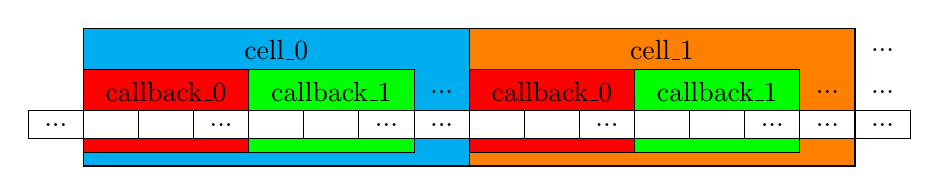
\begin{tikzpicture}[scale=0.7]
  % draw cells
  \draw[fill=cyan] (0,-0.5) rectangle ( 7,2);
  \draw[fill=orange]    (7,-0.5) rectangle (14,2);
  \node[align=center] at ( 3.5, 1.6) {cell\textunderscore{}0};
  \node[align=center] at (10.5, 1.6) {cell\textunderscore{}1};
  \node[align=center] at (14.5, 1.6) {...};
  
  % draw callbacks
  % cell_1
  \draw[fill=red]   (0,-0.25) rectangle (3,1.25);
  \draw[fill=green] (3,-0.25) rectangle (6,1.25);
  \node[align=center] at (1.5,0.85) {callback\textunderscore{}0};
  \node[align=center] at (4.5,0.85) {callback\textunderscore{}1};
  \node[align=center] at (6.5,0.85) {...};
  % cell_2
  \draw[fill=red]   ( 7,-0.25) rectangle (10,1.25);
  \draw[fill=green] (10,-0.25) rectangle (13,1.25);
  \node[align=center] at ( 8.5,0.85) {callback\textunderscore{}0};
  \node[align=center] at (11.5,0.85) {callback\textunderscore{}1};
  \node[align=center] at (13.5,0.85) {...};
  % beyond
  \node[align=center] at (14.5,0.85) {...};
  
  % draw contiguous memory
  \draw[fill=white] (-1,0) rectangle (15,0.5);
  \foreach \x in {0,...,14}
  \draw (\x,0) -- (\x,0.5);
  % cell_1
  \node[align=center] at ( 2.5,0.25) {...};
  \node[align=center] at ( 5.5,0.25) {...};
  \node[align=center] at ( 6.5,0.25) {...};
  % cell_2
  \node[align=center] at ( 9.5,0.25) {...};
  \node[align=center] at (12.5,0.25) {...};
  \node[align=center] at (13.5,0.25) {...};
  % beyond
  \node[align=center] at (-0.5,0.25) {...};
  \node[align=center] at (14.5,0.25) {...};
\end{tikzpicture}
\caption[Division of contiguous memory chunks for data transfer.]{Division of contiguous memory chunks for data transfer. Data is arranged according to the order of the cells. Registering \textit{pack} functions as callbacks allows to add multiple data chunks from different sources to each cell.}
\label{fig:memory}
\end{figure}

For the preparation of data buffers, all refinement indicators need to be terminally set. During both the packing and unpacking process, we determine whether cells will be or have been either refined, coarsened, or left untouched.

Simple data structures assigned on each cell can be easily packed and unpacked. However in case of \h-adaptation, data has to be transferred between parent cells and children. Depending on the context, it is upon the user's decision to provide an appropriate strategy, e.g., divide data of the parent cell equally on all children for refinement and sum data on all children for the parent cell for coarsening.

However, the transfer of complete finite element approximations is slightly more complicated. Here, we need to prepare data on each cell not only depending on the adaptation context, but also on the currently active finite element. In fact, we will already prepare data from the old mesh for the adapted grid in such a way that it just has to be unpacked on the new mesh. Regardless of whether \gls{cg} or \gls{dg} methods are employed, we will always store values of all \glspl{dof} on every cell to make sure that
all data is available on cells after transfer. %on locally owned cells, even if \glspl{dof} are owned by an adjacent ghost cell.
%potential ghost cells will have access to all necessary data.
\textcite{bangerth2012} developed an algorithm for transferring the solution across \h-adapted meshes in parallel, which will be expanded to work with \hp-adaptation in the remaining part of this section.

Once all adaptation indicators have been set, we know how cells will change during the execution of refinement and coarsening, so a corresponding \textit{pack} callback will look as follows: On all active cells which will not be coarsened, we interpolate or project all \gls{dof} values of the currently active finite element to the future finite element. On nonactive cells which have active children that will be coarsened, we interpolate or project all \gls{dof} values from the currently active finite elements on children to the future finite element of the parent cell, which is determined as the encapsulating finite element space among all children (see Sec.~\ref{sec:adaptation}).

This way, all data has been prepared for the new mesh and has to be distributed on it with the following \textit{unpack} callbacks after \hp-adaptation happened and all \glspl{dof} have been enumerated on the updated mesh. On every active cell that has not been changed or that is the result of coarsening, we simply extract all \gls{dof} values. If an active cell is the result of refinement, we extract all \gls{dof} values from its parent cell and interpolate them on the refined cells. All extracted \gls{dof} values are left to be copied to the global data container corresponding to the finite element approximation.

In the following, we give a detailed description of the algorithm implemented in the \dealii{} library which is tied to the usage of \pforest{} \textcite{p4est22} as an oracle and relies on features provided by it. Here, the \dealii{} triangulation is stored independently from the \pforest{} mesh.

In the application scope before adaptation is executed, users attach \textit{pack} callback functions to the triangulation and specify whether they qualify for fixed or variable size data transfer.

As soon as the user requests adaptation to be performed, all adaptation indicators will be carried over to the \pforest{} master mesh, which will be modified accordingly while maintaining the 2:1 mesh balance. The \dealii{} domain is left untouched.

We store a deep copy of the array of partition markers \parencite{burstedde2018} from the local \pforest{} object, which defines the global partition boundary allowing us to relate each cell to its corresponding subdomain. After repartitioning the \pforest{} master mesh, we know each cell's association to its subdomain on both the old and the adapted mesh with the corresponding partition markers, and thus source and destination processes for all \gls{mpi} communication.

%And store its global first quadrant shared data structure from which we can determine the association of all processors to each cell, repartition the mesh among all processors, and store the same data structure again. This way we know each cell's association to a processor on both meshes. \parencite{burstedde2018}

%With the new global first quadrant data, we know for each cell which processes owned it on the old and the new mesh. We can thus perform the actual transfer as follows.

Comparing the meshes of the updated \pforest{} object with the \dealii{} triangulation lets us identify how cells have changed.
%This way, we can compare both and determine how cells have changed in the adaptation process.
With this information, we are able to prepare data from the old mesh for the new one. We create the contiguous memory buffers for fixed size and variable size data transfer, respectively, by triggering all callback functions that return buffers for the particular data on each cell. In addition, we will store how cells have changed with a corresponding flag and write it to the fixed size buffer.

We determine the sizes of every cell's data pack in each buffer. For fixed size data, we verify the equality of their size on all cells. We store a list with the data size of every cell from the variable size buffer. After that, the fixed size data buffer and the list of sizes from the variable size buffer will be communicated via the optimized fixed size transfer function provided by \pforest{} \parencite{burstedde2018}. Last, the variable size data buffer will be transferred using the analogously optimized function after the list of sizes is available. %on all processes.

%We will communicate the fixed size data buffer and a list of all sizes from the variable size data buffer via the optimized fixed size transfer function provided by \pforest{} \parencite{burstedde2018}. In a next step, variable size data will be transferred after the individual sizes are available.

%We could also send the variable data sizes with the fixed size data transfer. However for convenience, we keep it like this.

After adaptation has been performed and all data has been communicated, the user is left to reinitialize all data structures according to the updated mesh and \textit{unpack} the transferred data into them.

%We came up with the following code in application scope to perform data transfer across meshes: We will first register data to be transferred. Storing function pointers that deal with packing required data. We distinguish between fixed and variable size data.
%
%\begin{enumerate}
%\item Register.
%\item Prepare contiguous memory blocks.
%\item Perform fixed size data transfer.
%\item Perform fixed size data transfer for variable sizes.
%\item Perform variable size data transfer.
%\item Unpack data.
%\end{enumerate}

%We build continguous memory buffers for both fixed and variable size transfer, and store each size of the latter. Then, we transfer both the fixed size buffer and all sizes via fixed sized transfer. After that, we transfer the variable size transfer useing all sizes.

%When mesh is about to be

With this feature, we are able to send all sorts of cell-related data across adapted meshes, e.g., particle data, quadrature point data, and finite element approximations. Further, we use the above algorithm to transfer active finite element indices internally. To be more precise, future finite element indices will be sent and unpacked as active finite element indices on the adapted mesh.

These contiguous memory chunks can also be used for the purpose of serialization. In case the program shall be interrupted and resumed at a later stage, data will be dumped to the file system. We will create two separate files, each containing either fixed size or variable size data.

Therefore, we need to determine the offset at which each process is supposed to write its local memory buffer into a global contiguous file. Thus, each process needs to know how much memory all preceding processes occupy. For fixed size data, this offset simply translates to the global index of the first cell on this process times the data size per cell. The global index can be determined from the array of partition markers of the \pforest{} object \parencite{burstedde2018}. However, in case of variable size data, we need to determine the offset with a prefix sum over the local buffer sizes of all preceding processes using \texttt{MPI\_Exscan} \textcite{mpi31}.

To resume the program successfully, we also need to store information about the data size of every cell, which we will prepend to the actual data in each file. In case of fixed size data, an integer corresponding to the data size per cell will be stored. For variable size data, we will collectively write the data size of every local cell in the global file, where each process's offset is determined by the global index of the first cell times the size of an integer.

Finally with this information, we can write all data collectively to the file system using \texttt{MPI\_File\_write\_at}, which can later be read from via \linebreak \texttt{MPI\_File\_read\_at} \textcite{mpi31}. For the serialization of the global mesh structure, we use the provided save and load functions of \pforest{}.

%With array of partition markers of the \pforest{} object \parencite{burstedde2018} combined with information about each cell's data size, we are able to determine the offset from the starting address that each processor needs to dump his data by a prefix sum over the cumulated data sizes.

%stores all cells in a consecutive order and partitions them, thus a sequence of all local cells across all processors

%to determine

%We need to find starting proc. Since we know the starting at the position of the global index of the first cell of the processor until the cumulated sum of the sizes on all locally owned cells.

Since all memory is written contiguously and the order of cells on the space-filling curve is independent of the partitioning, we can resume the program with a different number of processes than used during serialization.

%The preparation of data to be transferred and unpacking of transferred data has been realized in the \texttt{parallel::distributed::SolutionTransfer} \todo{cite} and \texttt{parallel::distributed::CellDataTransfer} classes within the \dealii{} library. The \texttt{parallel::distributed::Triangulation} \todo{cite} has been expanded by the preparation of the contiguous memory buffers and the execution of the transfer via \pforest{}.